
\documentclass[9pt]{beamer}
%\makeatletter
%\def\beamer@calltheme#1#2#3{%
%	\def\beamer@themelist{#2}
%	\@for\beamer@themename:=\beamer@themelist\do
%	{\usepackage[{#1}]{\beamer@themelocation/#3\beamer@themename}}}
%
%\def\usefolder#1{
%	\def\beamer@themelocation{#1}
%}
%\def\beamer@themelocation{}

%\usefolder{../config}

\usetheme[
block=fill,
titleformat=regular,
progressbar=frametitle
]{metropolis}
%\metroset[everytitleformat=regular] % regular, lowercase, uppercase ]
%\metroset[inner/block=fill]

%\setbeameroption{show notes} 
\usepackage{booktabs}
\usepackage[scale=2]{ccicons}

\usepackage{pgfplots}
\usepgfplotslibrary{dateplot}


%\ Hrvatski znakovi
\usepackage[utf8]{inputenc}
\usepackage[T1]{fontenc}
\usepackage[croatian]{babel}
\usepackage{todonotes}
\usepackage{amsmath}
\usepackage{amsfonts}
\selectlanguage{croatian} % american ngerman
\usepackage{todonotes}

% Koristenje Latin modern fonta
% Bez toga na nekim racunalima baca
% err: Font <taj i taj> at <mala velicina, npr4.0pt> not loadable: Metric (TFM) file not found. \end{frame}
\usepackage{lmodern}


\definecolor{RoyalBlue}{cmyk}{1, 0.50, 0, 0}
%\usepackage{natbib}
%\usepackage{bibentry}
\usepackage{scrextend}
\usepackage{hyperref}
%\usepackage[pdfa=true]{hyperref}
\hypersetup{%
    %draft, % = no hyperlinking at all (useful in b/w printouts)
    %colorlinks=true, 
    linktocpage=true, pdfstartpage=3, pdfstartview=FitV,%
    % uncomment the following line if you want to have black links (e.g., for printing)
    %colorlinks=false, linktocpage=false, pdfborder={0 0 0}, pdfstartpage=3, pdfstartview=FitV,% 
    breaklinks=true, pdfpagemode=UseNone, pageanchor=true, pdfpagemode=UseOutlines,%
    plainpages=false, bookmarksnumbered, bookmarksopen=true, bookmarksopenlevel=1,%
    hypertexnames=true, pdfhighlight=/O,%nesting=true,%frenchlinks,%
    %urlcolor=webbrown, linkcolor=RoyalBlue, citecolor=webgreen, %pagecolor=RoyalBlue,%
    %urlcolor=Blue, linkcolor=Blue, citecolor=Red, %pagecolor=Black,%
    %pdftitle={\myTitle},%
    %pdfauthor={\textcopyright\ \myName, \myUni, \myFaculty},%
    pdfsubject={},%
    pdfkeywords={},%
    pdfcreator={pdfLaTeX},%
    pdfproducer={LaTeX with hyperref and classicthesis}, %
    unicode = true 
} 

%\usepackage[pdftex]{graphicx}
% declare the path(s) where your graphic files are
\graphicspath{{./}{./figures/}}


\newcommand{\executeiffilenewer}[3]{%
	\ifnum\pdfstrcmp{\pdffilemoddate{#1}}%
	{\pdffilemoddate{#2}}>0%
	{\immediate\write18{#3}}\fi%
}
\newcommand{\includesvg}[1]{%
	\executeiffilenewer{#1.svg}{#1.pdf}%
	{inkscape -z -C --file=#1.svg %
		--export-pdf=#1.pdf --export-latex}%
	\input{#1.pdf_tex}%
}


% http://tex.stackexchange.com/questions/83882/how-to-highlight-python-syntax-in-latex-listings-lstinputlistings-command

\usepackage{listings}
\usepackage{color}
\usepackage[semibold]{sourcecodepro}

% Default fixed font does not support bold face
\DeclareFixedFont{\ttb}{T1}{txtt}{bx}{n}{12} % for bold
\DeclareFixedFont{\ttm}{T1}{txtt}{m}{n}{12}  % for normal
% Custom colors
\definecolor{deepblue}{rgb}{0,0,0.5}
\definecolor{deepred}{rgb}{0.6,0,0}
\definecolor{deepgreen}{rgb}{0,0.5,0}


% Python style for highlighting
\newcommand\pythonstyle{\lstset{
		language=Python,
		basicstyle=\small\ttfamily,
		otherkeywords={self},             % Add keywords here
		keywordstyle=\small\ttfamily\color{deepblue},
		emph={MyClass,__init__},          % Custom highlighting
		emphstyle=\small\ttfamily\color{deepred},    % Custom highlighting style
		stringstyle=\color{deepgreen},
		frame=tb,                         % Any extra options here
		showstringspaces=false            % 
	}}
	
	
	% Python environment
	\lstnewenvironment{python}[1][]
	{
		\pythonstyle
		\lstset{#1}
	}
	{}
	
	% Python for external files
	\newcommand\pythonexternal[2][]{{
			\pythonstyle
			\lstinputlisting[#1]{#2}}}
	
	% Python for inline
	\newcommand\pythoninline[1]{{\pythonstyle\lstinline!#1!}}

% \includeonlyframes{current}

%\documentclass[ucs]{beamer}
%\usetheme[menuwidth={0.3\paperwidth}]{erlangen}
%\setbeamercovered{transparent=20} 

\usepackage{amsmath,amsfonts,amsthm,amssymb}
\usepackage{setspace}
\usepackage{Tabbing}
\usepackage{fancyhdr}
\usepackage{lastpage}
\usepackage{extramarks}
\usepackage{chngpage}
\usepackage{soul,color}
\usepackage{graphicx,float,wrapfig}
\usepackage{xcolor}
\usepackage[normalem]{ulem}
\usepackage{mathtools}

\definecolor{erlangenlyellow}{RGB}{123, 25, 121}
%\usepackage[utf8x]{inputenc}
%\usepackage{default}
%\usepackage[T1]{fontenc}

\usepackage{verbatim}
\usepackage{listings}


\usepackage{subcaption}
\usepackage{lmodern}

\title{Teksture, sjene i sve između}

% \subtitle{ Yet, it doesn't seem so clear to me anymore…?}
\subtitle {Chao ab ordo}
\institute{Računalna grafika}


\begin{document}
\begin{frame}
 \titlepage
\end{frame}

%\begin{frame}{Sadržaj}
%  \tableofcontents
%  % You might wish to add the option [pausesections]
%\end{frame}
% \section{Uvod}
\section{Bump i displacement preslikavanje}
\begin{frame}{Bump mapping}
	\begin{block}{Problemi}
		\begin{itemize}
			\item Dodavanje teksture na glatku površinu rezultira glatkom površinom.
			\item Korištenje grube teksture u cilju prikaza grube površine nije dobra ideja.
			\item Grube površine bi trebale imati dodanu malu nasumičnu komponentu u normali, a time i u smjeru refleksije svjetla.
		\end{itemize}
	\end{block}
	\begin{itemize}
		\item Perturbacija normale površine
		\item Za svaku točku na površini $\mathbf{S}$, parcijalne derivacije su $\mathbf{S}_u$ i $\mathbf{S}_v$. 
		\item Odnosno: $\mathbf{n} = \mathbf{S}_u \times\mathbf{S}_v$
	\end{itemize}
\end{frame}	
%
\begin{frame}{Bump mapping}
	\begin{block}{}
		Nova ploha je definirana sa $S'(u,v) = S(u,v) + P(u,v)\frac{n}{|n|}$ \\
		gdje je $P(u,v)$ funkcija perturbacije u smjeru normale osnovne plohe, zadaje se analitički ili tablično\\
		Rezultirajuća normala je $\mathbf{n'} = \mathbf{S'}_{u} \times \mathbf{S'}_{v}$ 
	\end{block}
	
	\begin{block}{Konačno}
		$$n' = n + \frac{P_{u}(\mathbf{n} \times \mathbf{S}_{v})}{|n|} + \frac{P_{v}(\mathbf{S}_{u} \times \mathbf{n})}{|n|}$$
	\end{block}
\end{frame}
%

%
\begin{frame}{Displacement mapping}
	Vrijednosti teksture su vrijednosti pomaka geometrije u smjeru normale.
	\begin{center}
		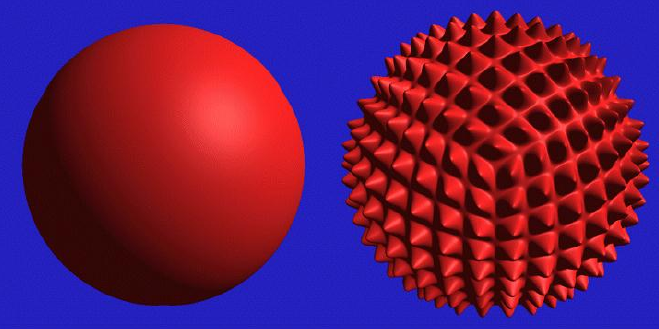
\includegraphics[width=2.5cm]{slike/displacement_map.png}
	\end{center}
	\begin{block}{}
		Bump mapping općenito ne zahtijeva puno resursa. Displacement mapping zahtijeva više resursa tijekom
		inicijalizacije i manipulacije, ali kako se računanje odvija tijekom postavljanja scene, ne povećava vrijeme renderiranja, dok bump mapping povećava vrijeme renderiranja iz razloga što pokreće novi shader proces.
	\end{block}
	
	
\end{frame}
%
%\begin{frame}{Bump vs Displacement mapping}
%	\begin{block}{Primjena Displacement mapping}
%		\begin{itemize}
%			\item tereni
%			\item animacija travnatih i šumovitih područja
%			\item valovi vodenih i sličnih površina
%			\item animacija vatre, dima, oblaka ili sličnih čestičnih volumena
%		\end{itemize}
%	\end{block}
%	
%	\begin{block}{Primjena Bump mapping}
%		\begin{itemize}
%			\item realizam tekstura - koža itd.
%			\item dodavanje malih detalja objektu
%		\end{itemize}
%	\end{block}
%\end{frame}
%
\begin{frame}{Bump vs Displacement mapping contd.}
	\begin{center}
		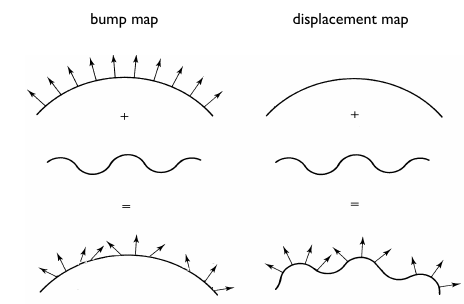
\includegraphics[width=10cm]{slike/03_bump_vs_displacement_mapping.png}
	\end{center}
\end{frame}

\begin{frame}{Bump mapping contd.}
	
	\begin{columns}[t]
		\begin{column}{5cm}
			\begin{center}
				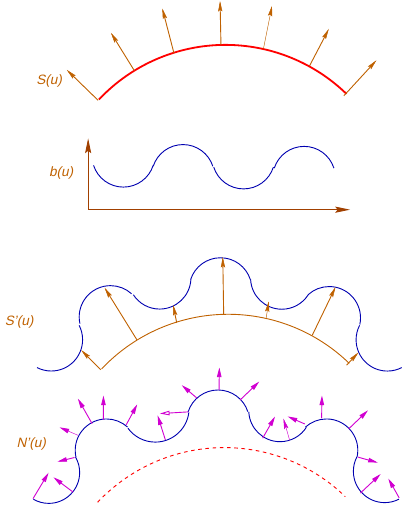
\includegraphics[width=5cm]{slike/03_bump_mapping.png}
			\end{center}
		\end{column}
		\begin{column}{7cm}
			\begin{center}
				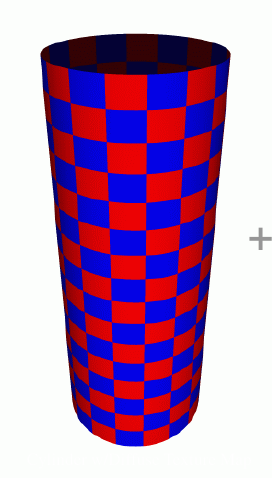
\includegraphics[width=1.8cm]{slike/bump_01.png}
				
\includegraphics[width=1.8cm]{slike/bump_02.png}
				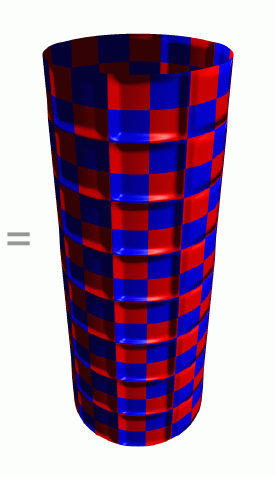
\includegraphics[width=1.8cm]{slike/bump_03.png}
			\end{center}
			\begin{center}
				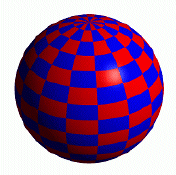
\includegraphics[width=1.8cm]{slike/bump_01_01.png}
				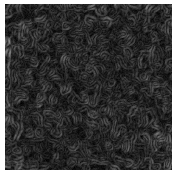
\includegraphics[width=1.8cm]{slike/bump_02_02.png}
				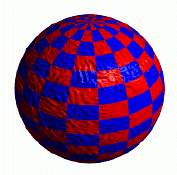
\includegraphics[width=1.8cm]{slike/bump_03_03.png}
			\end{center}
		\end{column}
	\end{columns}
\end{frame}

\begin{frame}{Bump vs Displacement mapping contd.}
	\begin{center}
		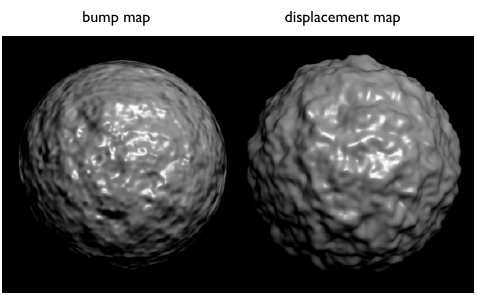
\includegraphics[width=10cm]{slike/03_bump_vs_displacement_mapping_a.png}
	\end{center}
\end{frame}



\begin{frame}{Bump/Normal mapping}
	Problem:
	\begin{center}
		
\includegraphics[width=8cm]{slike/normal_mapping_surfaces.png}
	\end{center}
	\begin{center}
	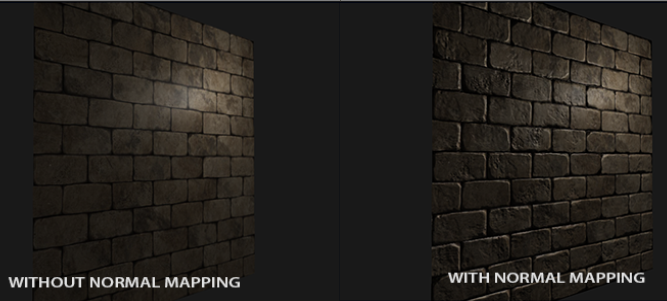
\includegraphics[width=11cm]{slike/normal_mapping_compare.png}
	\end{center}
\end{frame}

\begin{frame}{Normale}
	\begin{itemize}
		\item Boja: $(\mathrm{r}, \mathrm{g}, \mathrm{b})$
		\item Normala: $(x, y, z)$
		\item Normale možemo spremiti u sliku
		\item $x$ u $u$ smjeru, $y$ u $v$ smjeru, $z$ smjer: $u\times v$
	\end{itemize}
	
	\begin{center}
		
\includegraphics[width=4cm]{slike/normal_mapping_normal_map.png}
	\end{center}
\end{frame}
\begin{frame}{Još jedan problem}
	Normale iz teksture odgovaraju globalnom koordinatnom sustavu.
	
	\begin{center}
		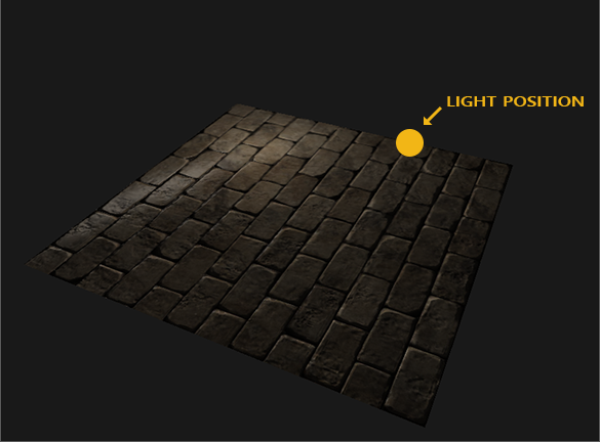
\includegraphics[width=4cm]{slike/normal_mapping_ground.png}
		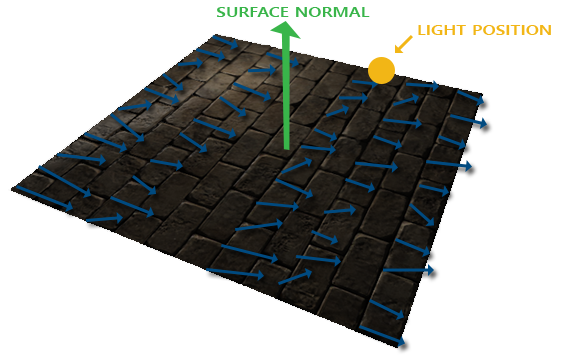
\includegraphics[width=5cm]{slike/normal_mapping_ground_normals.png}
	\end{center}
\end{frame}
\begin{frame}{Tangente i normala}

	\begin{columns}
		\begin{column}{0.7\textwidth}
			\begin{itemize}
				\item Koordinate verteksa: $P_1$,$P_2$ i $P_3$
				\item Znamo $(u, v)$ za svaki verteks, $P_1$,$P_2$ i $P_3$
				\item $E_1 = \Delta U_1 T +\Delta V_1 B$, $E_2 = \Delta U_2 T +\Delta V_2 B$
			\end{itemize}
			\begin{align*}
			(E_{1x}, E_{1y}, E_{1z}) = \Delta U_1(T_x, T_y, T_z) + \Delta V_1(B_x, B_y, B_z) \\
			(E_{2x}, E_{2y}, E_{2z}) = \Delta U_2(T_x, T_y, T_z) + \Delta V_2(B_x, B_y, B_z)
			\end{align*}
			ili
			\begin{align*}
			\begin{pmatrix}
				E_{1x} & E_{1y} & E_{1z} \\
				E_{2x} & E_{2y} & E_{2z}
			\end{pmatrix}
			=
			\begin{pmatrix}
			\Delta U_1 & \Delta V_1 \\
			\Delta U_2 & \Delta V_2
			\end{pmatrix} 
			\begin{pmatrix}
			T_x & T_y &  T_z \\
			B_x & B_y &  B_z
			\end{pmatrix} 
			\end{align*}
		\end{column}
		\begin{column}{0.3\textwidth}
				\begin{center}
				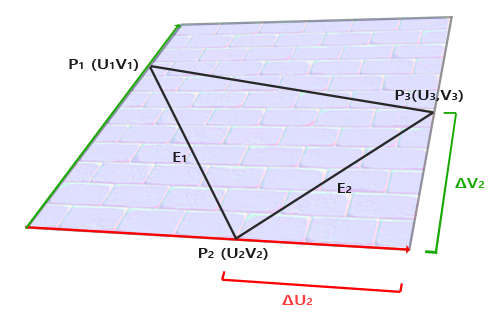
\includegraphics[width=3cm]{slike/normal_mapping_surface_edges.png}
			\end{center}
			\begin{center}
				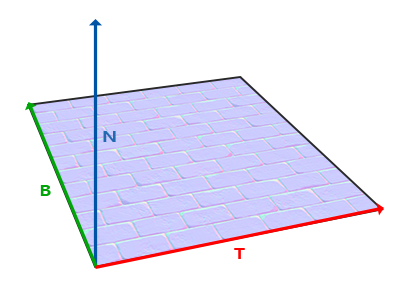
\includegraphics[width=3cm]{slike/normal_mapping_tbn_vectors.png}
			\end{center}
		\end{column}
	\end{columns}
	Na kraju dobijemo:
	\begin{align*}
	\begin{pmatrix}
	T_x & T_y &  T_z \\
	B_x & B_y &  B_z
	\end{pmatrix} = 
	\frac{1}{\Delta U_1\Delta V_2 - \Delta U_2\Delta V_1}
	\begin{pmatrix}
	\Delta V_2 & -\Delta V_1 \\
	-\Delta U_2 & \Delta U_1
	\end{pmatrix} 
	\begin{pmatrix}
	E_{1x} & E_{1y} & E_{1z} \\
	E_{2x} & E_{2y} & E_{2z}
	\end{pmatrix}
	\end{align*}
\end{frame}
\begin{frame}{Tangente i normala, contd.}
	\begin{align*}
	T_x = \frac{1}{\Delta U_1\Delta V_2 - \Delta U_2\Delta V_1} (\Delta V_2 E_{1x}-\Delta V_1 E_{2x}) \\
	T_y = \frac{1}{\Delta U_1\Delta V_2 - \Delta U_2\Delta V_1} (\Delta V_2 E_{1y}-\Delta V_1 E_{2y}) \\
	T_z = \frac{1}{\Delta U_1\Delta V_2 - \Delta U_2\Delta V_1} (\Delta V_2 E_{1z}-\Delta V_1 E_{2z})
	\end{align*}
	
	$B$ se može izračunati i ovako:
	\begin{align*}
	B = N \times T
	\end{align*}
\end{frame}
\begin{frame}{Parallax mapping}
	\begin{itemize}
		\item Skoro displacement mapping
	\end{itemize}
	
	\begin{center}
		
\includegraphics[height=4cm]{slike/parallax_mapping_height_map.png}
		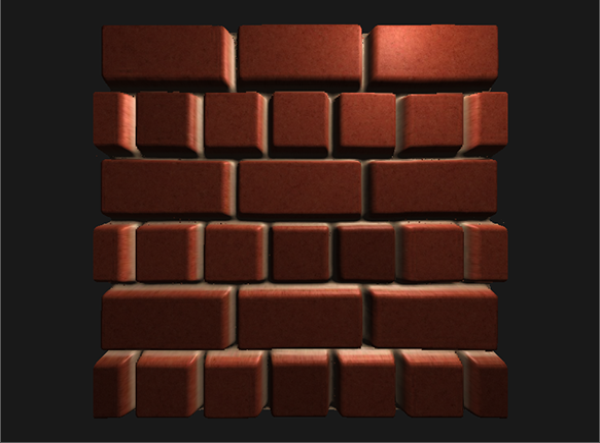
\includegraphics[height=4cm]{slike/parallax_mapping_plane_heightmap.png}
	\end{center}

\end{frame}
\begin{frame}{Parallax mapping, ideja}
	Nije dobro:
	\begin{center}
		
\includegraphics[width=6cm]{slike/parallax_mapping_plane_height.png}
	\end{center}
	Bolje:
	\begin{center}
	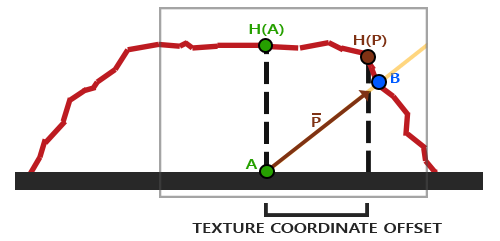
\includegraphics[width=5cm]{slike/parallax_mapping_scaled_height.png}
	\end{center}
\end{frame}

\begin{frame}{Parallax mapping, problem}
	Nije idealno rješenje	
	\begin{center}
		
\includegraphics[width=4cm]{slike/parallax_mapping_incorrect_p.png}
	\end{center}

\end{frame}

\begin{frame}{Parallax mapping, ideja}
	\begin{columns}
		\begin{column}{0.4\textwidth}
				Height map: ($0$ maksimalna visina, $1$ minimalna visina)
			\begin{center}
				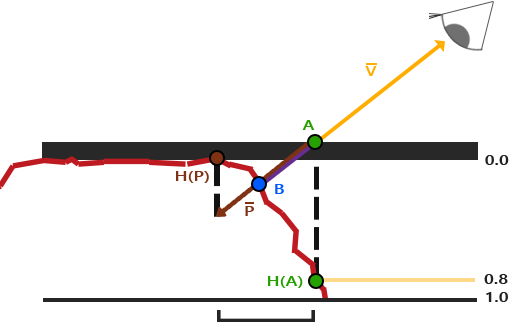
\includegraphics[width=4cm]{slike/parallax_mapping_depth.png}
			\end{center}
		\end{column}
		\begin{column}{0.6\textwidth}
				\begin{align*}
			P_x = s H(A)\frac{V_x}{V_z} \\ 
			P_y = s H(A)\frac{V_y}{V_z}
			\end{align*}
			Ovdje je $s=\mathrm{const.}$ 
			\begin{align*}
			H(P)_x = A_x - P_x \\
			H(P)_y = A_y - P_y
			\end{align*}
			Treba znati: $\vec{V}$ ne normaliziran, pa je $\vec{V}_z \in \left[0, 1\right]$ \\
			Što ako je $\vec{V}$ skoro paralelan s povšinom?
		\end{column}
	\end{columns}
\end{frame}

\section{Depth spremnik}
\begin{frame}{Depth spremnik, ideja}
	\begin{figure}
		\centering
		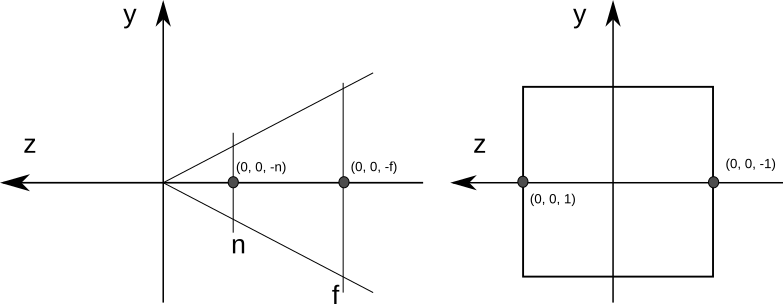
\includegraphics[width=0.7\textwidth]{slike/p04_07.png}
	\end{figure}
	\begin{itemize}
		\item Homogene koordinate čuvaju sve odnose, npr. depth
		\item Dovoljno je gledati samo $z$ koordinatu
	\end{itemize}

	\begin{itemize}
		\item Za svaki piksel: odgovarajuća dubina, inicijalno najmanji broj
		\item Izračunati $z$ iz \text{image space}
		\item Provjeriti ako je veći od postojećeg ($1$ crtati, $0$ ništa)
		\item Jedan \texttt{if} uvjet!
	\end{itemize}
\end{frame}

\begin{frame}{Implementacija}

	\begin{itemize}
		\item $Z$ spremnik sadrži vrijednosti od $0$ do $1$
		\item $z$ vrijednosti mogu biti bilo koja vrijednost između \textit{near} i \textit{far}
	\end{itemize}
Prvi pokušaj:
	\begin{align*}
		F_d = \frac{z-near}{far - near}
	\end{align*}
	\begin{figure}
		\centering
		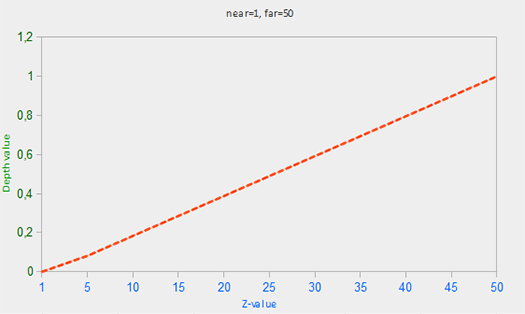
\includegraphics[width=0.4\textwidth]{slike/depth_linear_graph.png}
	\end{figure}
\end{frame}

\begin{frame}{Implementacija, contd.}
	\begin{itemize}
		\item Dubina u projekciji je proporcionalna sa $1/z$
		\item za $1 < z < 2$, $1 > F_d > 0.5$
		\item za $50 < z < 100$, $0.02 > F_d > 0.01$
	\end{itemize}
	Ispravnije:
	\begin{align*}
	F_d = \frac{1/z-1/near}{1/far - 1/near}
	\end{align*}
		\begin{figure}
		\centering
		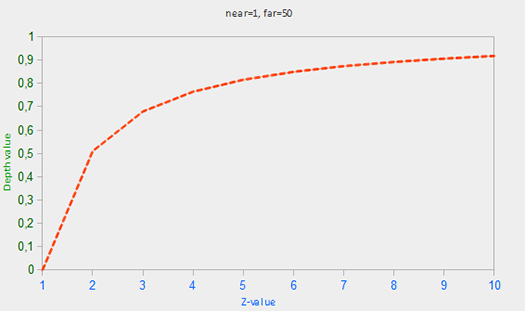
\includegraphics[width=0.4\textwidth]{slike/depth_non_linear_graph.png}
	\end{figure}
\end{frame}
\begin{frame}{Za kraj, $Z$ fighting}
	\begin{itemize}
		\item Što ako su dvije površine toliko blizu jedna drugoj da su razlike manje od rezolucije \textit{float} spremnika?
		\item Kreira se dovoljno mali \textit{offset} između površina
		\item $far$ i $near$ se postave što je moguće bliže jedna drugoj
		\item Primjer: pod i mrlja na podu, dvije površine s istim $z$ vrijednostima
	\end{itemize}
	
	\begin{figure}
		\centering
		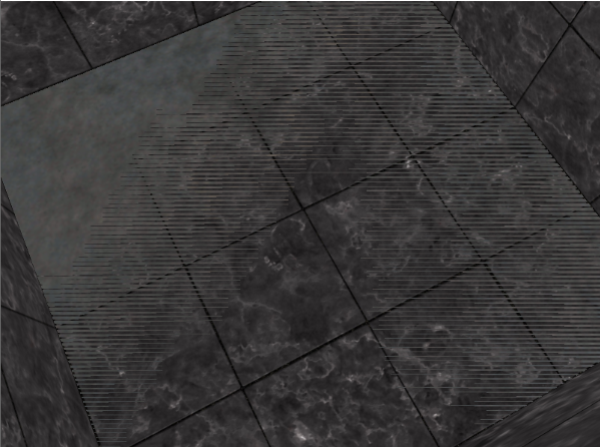
\includegraphics[width=0.4\textwidth]{slike/depth_testing_z_fighting.png}
	\end{figure}
\end{frame}

\section{Uklanjanje skrivenih linija i površina}
\begin{frame}{Problem}
	\begin{center}
		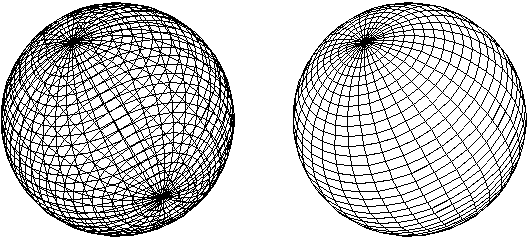
\includegraphics[height=4cm]{./slike/meshSpheres.png}
	\end{center}
\end{frame}

\begin{frame}{Motivacija}
	\begin{figure}
		\centering
		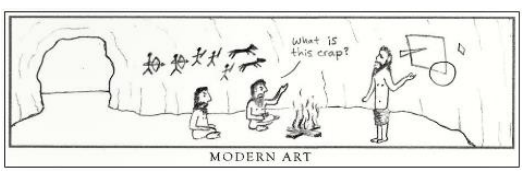
\includegraphics[width=0.8\linewidth]{./slike/modern_art}
		%		\caption{}
		%		\label{fig:modernart}
	\end{figure}
	
\end{frame}
\begin{frame}{Uklanjanje skrivenih linija i površina}
	\begin{block}{Osnove postupaka uklanjanja skrivenih linija i površina}
		\begin{itemize}
			\item geometrijska izračunavanja – uspostavljaju odnos između poligona, bridova i točaka (“containment test”)
			\item geometrijsko uređivanje (“geometric sorting”)
			\item postupci pretraživanja (“search algorithms”)
			\item međusoban ovisnost i obilježja (“coherence”)
		\end{itemize}
	\end{block}
\end{frame}

\begin{frame}{Uklanjanje contd.}
	\begin{block}{Određivanje vidljivosti}
		\begin{itemize}
			\item uklanjanje objekata izvan piramide pogleda (dijelova poligona)
			\item uklanjanje stražnjih pogona (eng. back face culling)
			\item brzi, jednostavni postupci za rješavanje trivijalnih slučajeva (npr. Min-maks provjera)
			\item promjena složenosti prikaza ovisno o udaljenosti (eng. LOD-level of detail)
		\end{itemize}
	\end{block}
	
	\begin{block}{Gruba podjela:}
		\begin{itemize}
			\item postupci u prostoru objekta 3D
			\item postupci u prostoru slike (projekcije) 2D
		\end{itemize}
	\end{block}
\end{frame}

\begin{frame}{Uklanjanje contd.}
	\begin{block}{Slični postupci:}
		\begin{itemize}
			\item odsijecanje (engl. clipping)
			\item  detekcije sudara tj. kolizije (engl. collision detection)
			\item bačene sjene
		\end{itemize}
	\end{block}
	\begin{block}{Geometrijska izračunavanja}
		Čine osnovu u postupcima uklanjanja skrivenih linija i poligona (u prostoru projekcije ili scene)
		\begin{itemize}
			\item položaj točke prema pravcu ili ravnini, prema poligonu ili tijelu
			\item položaj dužine prema pravcu ili ravnini, prema  poligonu ili tijelu
			\item Booleove operacije dvaju tijela (solid modelling)
			\item određivanje orijentacije poligona (u projekciji)
		\end{itemize}
	\end{block}
\end{frame}
%\begin{frame}{}
%	\begin{figure}
%		\centering
%		
\includegraphics[width=0.3\linewidth]{./slike/58mcs2}
%		%		\caption{}
%		%		\label{fig:modernart}
%	\end{figure}
%\end{frame}
\section{Poligon}
\begin{frame}{Poligon}
	Poligon se definira listom točaka $T_i$ koje su povezane bridovima $b_i$ na sljedeći način:
	\begin{align*}
	b_i \ldots \left\{ \begin{array}{cc}
	T_i, T_{i+i} & 0 < i < n \\
	Ti, T_0 & i = n
	\end{array}\right.
	\end{align*}
	Jednadžba pravca brida:
	\begin{align*}
	T_b= \left\{ \begin{array}{cc}
	(T_{i+i}-T_i)\lambda + T_i & 0 < i < n \\
	(T_0-T_i)\lambda + T_i & i = n
	\end{array}\right.
	\end{align*}
	Ovdje je $T_b$ proizvoljna točka pravca, ali samo za  $0 \leq \lambda \leq 1$, točka pripada bridu.
\end{frame}

\begin{frame}{Poligon}
	Pravac se dobije i kao vektorski produkt dvije točke:
	\begin{align*}
	T_i \times T_{i+1} & = \begin{bmatrix}
	\vec{i} & \vec{j}  & \vec{k}\\ 
	T_{i, 1} & T_{i, 2} & 1 \\
	T_{i+1, 1} & T_{i+1, 2} & 1 \end{bmatrix} \\
	& = \begin{bmatrix}
	\vec{i} & \vec{j}  & \vec{k}
	\end{bmatrix} 
	\begin{bmatrix}
	T_{i, 2} - T_{i+1, 2}\\
	-(T_{i, 1} - T_{i+1, 1})\\
	T_{i,1}T_{i+1, 2}- T_{i,2}T_{i+1, 1} 
	\end{bmatrix} \\
	& = \begin{bmatrix}
	\vec{i} & \vec{j}  & \vec{k}
	\end{bmatrix}B_i \quad 0 < i < n
	\end{align*}
	\begin{align*}
	T_i \times T_0 & = \begin{bmatrix}
	\vec{i} & \vec{j}  & \vec{k}\\ 
	T_{i, 1} & T_{i, 2} & 1 \\
	T_{0, 1} & T_{0, 2} & 1 \end{bmatrix} \\
	& = \begin{bmatrix}
	\vec{i} & \vec{j}  & \vec{k}
	\end{bmatrix} 
	\begin{bmatrix}
	T_{i, 2} - T_{0, 2}\\
	-(T_{i, 1} - T_{0, 1})\\
	T_{i,1}T_{0, 2}- T_{i,2}T_{0, 1} 
	\end{bmatrix} \\
	& = \begin{bmatrix}
	\vec{i} & \vec{j}  & \vec{k}
	\end{bmatrix}B_i \quad i = n
	\end{align*}
	$B_i$ su koeficijenti pravca.
\end{frame}
\begin{frame}{Orijentacija vrhova poligona}
	\begin{columns}
		\begin{column}[t]{0.5\textwidth}
			CW
			\begin{figure}
				\centering
				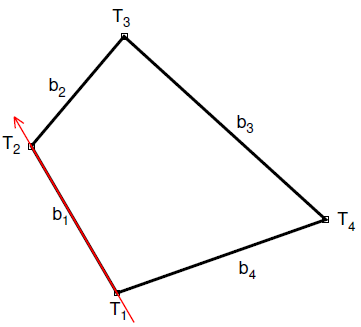
\includegraphics[width=0.8\textwidth]{slike/poligon_cw.png}
			\end{figure}
			\begin{align*}
			(\forall i) T_j \cdot B_i \leq 0 
			\end{align*}
		\end{column}
		\begin{column}[t]{0.5\textwidth}
			CCW
			\begin{figure}
				\centering		
				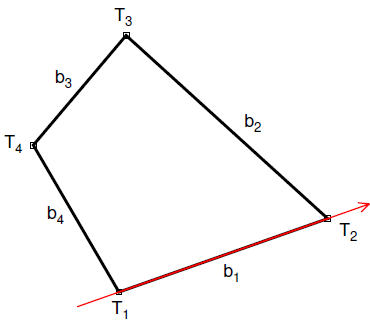
\includegraphics[width=0.8\textwidth]{slike/poligon_ccw.png}
			\end{figure}
			\begin{align*}
			(\forall i) T_j \cdot B_i \geq 0 
			\end{align*}
		\end{column}
	\end{columns}
	gdje je 
	\begin{align*}
	j = \left\{ \begin{array}{cc}
	j = i+2, & 0 < i < n-i \\
	j = i-n +2, & n-1 \leq i \leq n 
	\end{array}
	\right.
	\end{align*}
\end{frame}

\begin{frame}{Poligon konveksan?}
	\begin{columns}
		\begin{column}[t]{0.5\textwidth}
			CW
			\begin{figure}
				\centering
				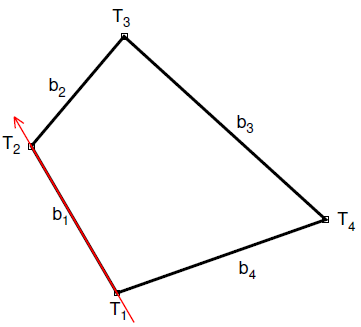
\includegraphics[width=0.8\textwidth]{slike/poligon_cw.png}
			\end{figure}
			Ako vrijedi 
			\begin{align*}
			(\exists i) T_j \cdot B_i < 0 ,
			\end{align*}
			Onda postoji barem jedan vrh takav da se nalazi ispod brida, odnosno, ako vrijedi za sve vrhove
			\begin{align*}
			(\forall i) T_j \cdot B_i \leq 0 
			\end{align*}
		\end{column}
		\begin{column}[t]{0.5\textwidth}
			CCW
			\begin{figure}
				\centering		
				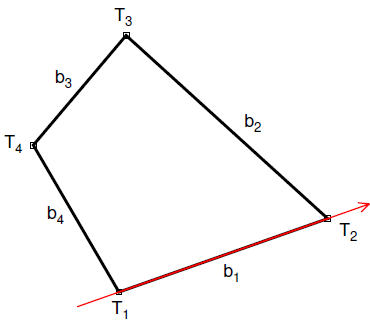
\includegraphics[width=0.8\textwidth]{slike/poligon_ccw.png}
			\end{figure}
			Ako vrijedi 
			\begin{align*}
			(\exists i) T_j \cdot B_i > 0 ,
			\end{align*}
			Onda postoji barem jedan vrh takav da se nalazi ispod brida, odnosno, ako vrijedi za sve vrhove
			\begin{align*}
			(\forall i) T_j \cdot B_i \geq 0 
			\end{align*}
		\end{column}
	\end{columns}	
\end{frame}
\begin{frame}{Poligon konveksan?}
	\begin{block}{tldr;}
		Poligon je konveksan ako vrijedi:
		\begin{align*}
		(\forall i) T_j \cdot B_i \leq 0
		\end{align*}
		ili
		\begin{align*}
		(\forall i) T_j \cdot B_i \geq 0 
		\end{align*}
	\end{block}
	\begin{block}{još jedna sitnica}
		Ako smo sigurni da je poligon konveksan, onda orijentaciju vrhova možemo testirati tako da ispitamo samo jednu točku sa jednim bridom.
	\end{block}
\end{frame}
\begin{frame}{Provjera odnosa točke i poligona}
	\begin{block}{Korištenje sume kuteva}
		\begin{itemize}
			\item ako je $\sum_{i} \alpha_{i} = 0$, $P_{t}$ je izvan poligona
			\item ako je $\sum_{i} \alpha_{i} = 2\pi$, $P_{t}$ je unutar poligona 
		\end{itemize}
	\end{block}
	
	\begin{block}{Koristimo skalarni produkt, samo za konveksne poligone}
		\begin{itemize}
			\item CW poligon: ako je $(\forall i) T_j \cdot B_i \geq 0$ točka je unutar poligona
			\item CCW poligon: ako je $(\forall i) T_j \cdot B_i \leq 0$ točka je unutar poligona 
		\end{itemize}
	\end{block}
\end{frame}

\section{Provjera normale}
\begin{frame}{Provjera normale}
	\begin{block}{Cilj}
		Ne iscrtavati stražnje poligone nekog geometrijskog tijela.
	\end{block}
	\begin{block}{Pretpostavke}
		\begin{itemize}
			\item Tijelo je opisano nizom poligona
			\item Tijelo je konveksno
			\item Vrhovi poligona su zadani u CCW smjeru
		\end{itemize}
	\end{block}
	\begin{block}{Posljedica}
		\begin{itemize}
			\item Normale gledaju iz tijela prema van
			\item Normala koja je \textit{od očišta} pripada stražnjem poligonu
		\end{itemize}
	\end{block}
\begin{center}
	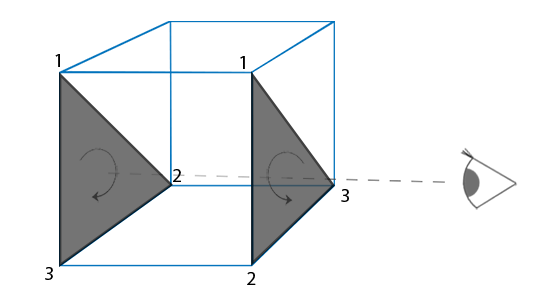
\includegraphics[height=2.5cm]{./slike/faceculling_frontback.png}
\end{center}
\end{frame}
\begin{frame}{Provjera normale}
	\begin{block}{Tehnikalije}
		\begin{itemize}
			\item Provjerava se kut koji zatvara normala poligona i vektor usmjeren iz središta poligona prema očištu
			\item poligon je stražnji ako $\vec{N}_P\cdot \cdot \vec{N} < 0$
			\item poligon je prednji ako $\vec{N}_P\cdot \cdot \vec{N} > 0$
			\item promatrač vidi poligon kao liniju $\vec{N}_P\cdot \cdot \vec{N} = 0$
		\end{itemize}
	\end{block}
	\begin{center}
		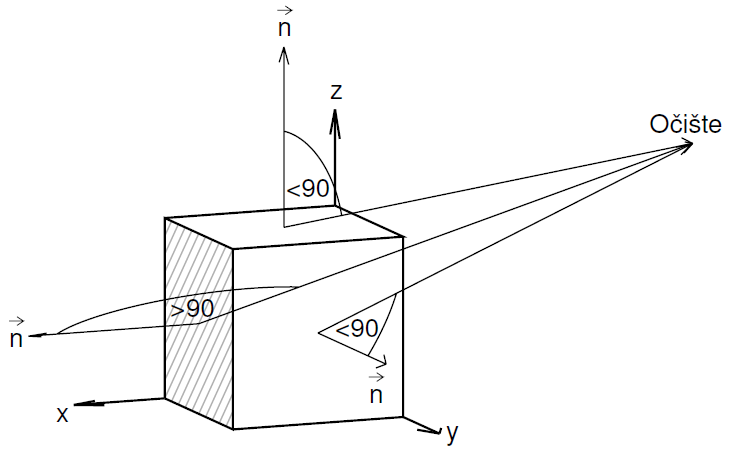
\includegraphics[height=3.5cm]{./slike/provjera_normala.png}
	\end{center}
\end{frame}

\begin{frame}{Provjera normale}
	\begin{block}{Drugi način}
		\begin{itemize}
			\item Kreiramo ravninu kojoj pripada poligon
			\item Uvrstimo položaj očišta u jednadžbu ravnine
			\item Ako je očište \textit{ispod}, poligon je stražnji
			\item Ako je očište \textit{iznad}, poligon je prednji
		\end{itemize}
		$\mathbf{T}\cdot \mathbf{R}$ - izrazi 2.39 iz skripte: $<0$ ispod, $>0$ iznad. 
	\end{block}
	
	\begin{block}{Problemi}
		Voditi računa o transformacijama normala kod perspektivne projekcije.
	\end{block}
\end{frame}

\section{Sjene}
\begin{frame}{Ideja}
	\begin{figure}
		\centering
		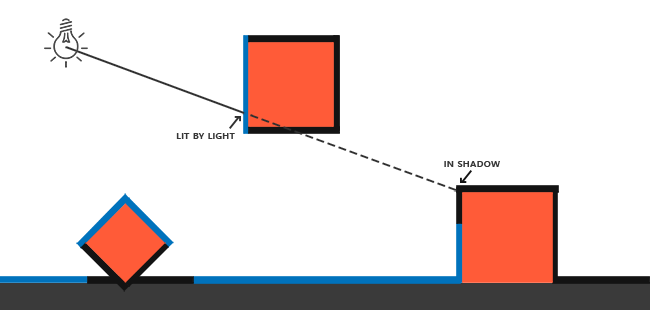
\includegraphics[width=0.8\textwidth]{slike/shadow_mapping_theory.png}
	\end{figure}
\end{frame}

\begin{frame}{Implementacija, 1. korak}
	\begin{figure}
		\centering
		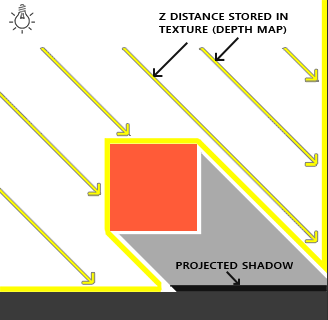
\includegraphics[width=0.3\textwidth]{slike/shadow_mapping_theory_spaces_left.png}
	\end{figure}
	\begin{itemize}
		\item Render scene iz perspektive svjelta
		\item Izračunati matricu transformacije iz perspektive svjetla
		\item Spremiti udaljenosti u teksturu (fragment shader)
		\item Udaljenosti se odnose na udaljenost od izvora svjetla do najbliže prepreke
	\end{itemize}
Drugi korak podrazumijeva računanje transformacijske matrice $\mathbf{T} = \mathbf{C}\mathbf{M}_p$ (treće predavanje)
\end{frame}	
\begin{frame}{Implementacija, 2. korak}
	\begin{figure}
		\centering
		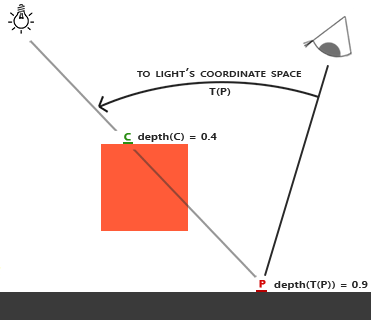
\includegraphics[width=0.3\textwidth]{slike/shadow_mapping_theory_spaces_right.png}
	\end{figure}
	\begin{itemize}
		\item Osim "normalnih" transformacija
		\item Pomnožiti svaki verteks s matricom $\mathbf{T}$ 
		\item Podijeliti sa $w$ da dobijemo $z$
		\item Ako je $z$ veći od vrijednositi u "shadow" teksturi, onda je objekt u sjeni
	\end{itemize}
\end{frame}	

\begin{frame}{Problemi, \text{shadow acne}}
	\begin{figure}
		\centering
		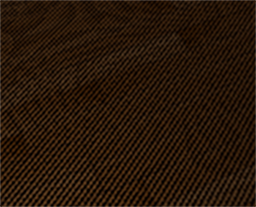
\includegraphics[width=0.25\textwidth]{slike/shadow_mapping_acne.png}
		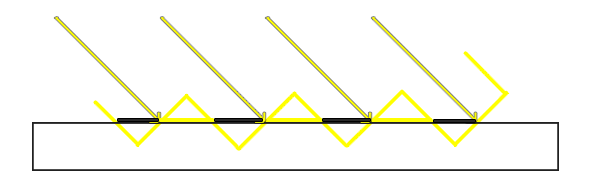
\includegraphics[width=0.45\textwidth]{slike/shadow_mapping_acne_diagram.png}
	\end{figure}
	\begin{itemize}
		\item "Shadow" spremnik je ograničen rezolucijom teksture
		\item Više fragmenata uzorkuje istu vrijednost iz  "shadow" spremnik
		\item Rješenje: pomaknemo površinu (ili vrijednosti sjene) za neku malu vrijednost ($\epsilon$, \textit{bias})
	\end{itemize}
\begin{figure}
	\centering
	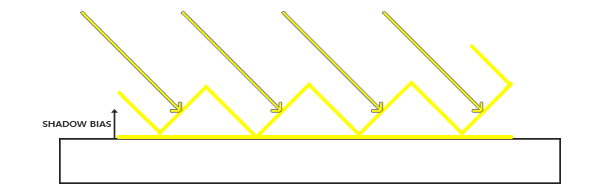
\includegraphics[width=0.45\textwidth]{slike/shadow_mapping_acne_bias.png}
\end{figure}
\end{frame}

\begin{frame}{Problemi, \text{peter panning}}
	Sada imamo drugi problem:
	\begin{itemize}
		\item U nekim situacijama $\epsilon$ može uzrokovati vidljivi pomak (\textit{offset}) sjene u odnosu na položaj objekta
		\item Rješenje: Render "shadow" mape samo sa stražnjim poligonima (tzv. \textit{front face culling})
	\end{itemize}
	\begin{figure}
		\centering
		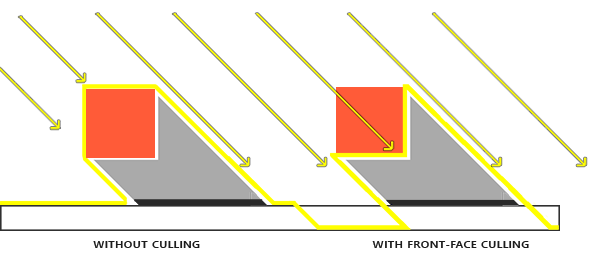
\includegraphics[width=0.7\textwidth]{slike/shadow_mapping_culling.png}
	\end{figure}
\end{frame}

\begin{frame}{Ortografska projekcija, ili?}
	Sada imamo drugi problem:
	\begin{itemize}
		\item Ortografska projekcija za \textit{directional} izvor svjetla
		\item Perspektivna projekcija za \textit{point} izvor svjetla
	\end{itemize}
	\begin{figure}
		\centering
		
\includegraphics[width=0.7\textwidth]{slike/shadow_mapping_projection.png}
	\end{figure}
\end{frame}

\begin{frame}{Što sa \textit{omnidirectional} svjetlom?}
	\begin{itemize}
		\item Ne koristi se 2D tekstura, već \textit{cube face} (S preslikavanje, kocka, 5. predavanje)
	\end{itemize}
\begin{figure}
	\centering
	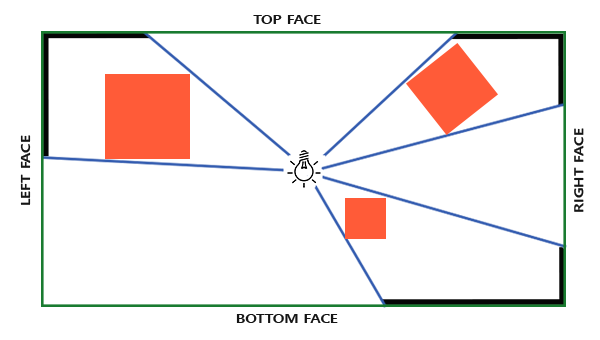
\includegraphics[width=0.7\textwidth]{slike/point_shadows_diagram.png}
\end{figure}
\end{frame}


\plain{Pitanja?}
\end{document}